%\section{Artificial Neural Networks}
\label{sec:ANN}
ANNs represent a type of computing based on the way that the brain
performs computations. It does not approach the complexity of the
brain; however, there are three similarities between biological and
artificial neural networks:

\begin{itemize}
	\item The basic unit of both systems -the neuron- is a very
	simple computational element that is highly
	interconnected.  

        \item The connections among those neurons determine the
	function of the network.

        \item Despite having a very simple set of rules of behaviour,
	when a neuron interacts with others, the global response of
	the system becomes much more complex.
\end{itemize}

The next sections explain how a biological neuron is modeled in order
to build artificial neural networks capable of solving complex
problems.

\subsection{Neuron model}
\label{subsec:neuronmodel}

As described in \secref{BNN}, a typical biological neuron has four
main regions: the soma, the axon, the dendrites and the
synapses. These parts are also be differentiated in an artificial
neuron. \figref{aneuronmodel} shows how a biological neuron is model
for ANNs.

\begin{figure}[!ht]
\centering
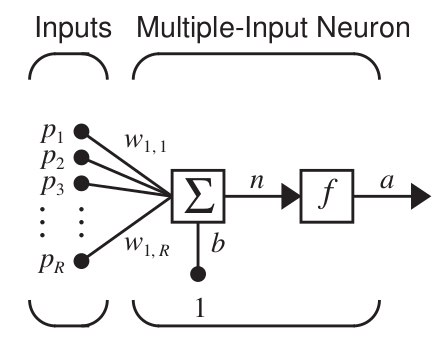
\includegraphics[width=0.5\textwidth]{images/neuronmodel.png}
\caption{Model of an artificial neuron inspired in a biological one}
\label{fig:aneuronmodel}
\end{figure}

In an artificial neuron, the \emph{inputs} $p_{k}, k=1,...,R$ are
multiplied by \emph{weights} $w_{k}$ and summed up together with the
optional constant \emph{bias} or \emph{offset} term $b$. The resulting
scalar $n$, often referred to as the \emph{net input}, goes into
the \emph{activation function} -also called \emph{transfer function}-
$f$, which produces the scalar neuron \emph{output} $a$.  Thus,
the \emph{output} of the neuron $i$
becomes \cite{Demuth:2014:NND:2721661}:

\begin{equation}
a_{i}=f_{i}(n_{i})=f_{i}(\sum_{k=1}^R w_{ik}p_{k}+b_{i})
\label{eq:expandedgeneralneuroneq}
\end{equation}

Relating this neuron model back to the biological neuron that we
discussed in \secref{BNN}, the set of \emph{inputs} $p_{k}$
corresponds to the dendritic tree, each \emph{weight} $w_{k}$ emulates
the strength of a synapse, the soma is represented by the summation
and the \emph{activation function} $f$, and the neuron \emph{output}
$y$ represents the signal on the axon.

The behavior of the neuron depends strongly on the particular
activation function that is chosen. Then the scalar parameters $w_{k}$
and $b$ will be adjusted by some learning rule so that the neuron
input/output relationship meets some specific goal.

The activation function $f$ may be a linear or a nonlinear function of
the net input $n$.  A particular function is chosen to satisfy some
specification of the problem that the neuron is attempting to
solve. The following functions are some of the ones often used in
ANNs \cite{Demuth:2014:NND:2721661}:

\begin{description}
	\item{\textbf{\emph{Hard limit} or \emph{Step} function}\hfill \\

	It sets the output of the neuron to 0 if the function argument
	is less than 0, or 1 if its argument is greater than or equal
	to 0. Its symetric version follows the expression:

		\begin{equation}
		a = f(n) =
  			\begin{cases}
    			-1 & \text{if } n < 0\\
    			1 & \text{if } n \geq 0
  			\end{cases}
		\label{eq:hardlimit}
		\end{equation}

	This activation function is commonly used to create neurons
	that classify inputs into two distinct categories.

	}
	\item{\textbf{\emph{Linear} function}\hfill \\

	The output of a linear transfer function is equal to its input
	($a=f(n)=n$). This simple function have some variations that
	are often used in artificial neurons:

	\begin{itemize}
		\item \emph{Positive linear} function, which guarantees to take nonnegative values according to the equation:
		\begin{equation}
		a = f(n) =
  			\begin{cases}
    			0 & \text{if } n < 0\\
    			n & \text{if } n \geq 0
  			\end{cases}
		\label{eq:positivelinear}
		\end{equation}

		\item \emph{Saturating linear} function, whose symmetric version is mathematically expressed as:
		\begin{equation}
		a = f(n) =
  			\begin{cases}
    			-1 & \text{if } n < -1\\
    			n & \text{if } -1 \leq n \leq 1\\
    			1 & \text{if } n > 1
  			\end{cases}
		\label{eq:saturatinglinear}
		\end{equation}
	\end{itemize}
	}
	\item{\textbf{\emph{Log-Sigmoid} function}\hfill \\
	This activation function takes the input (which may have any value between plus and minus infinity) and squashes the output into the range 0 to 1, according to the expression:

	\begin{equation}
	a = f(n) = \frac{1}{1+e^{-n}}
	\label{eq:logsig}
	\end{equation}

	The log-sigmoid function is commonly used in multilayer
	networks that are trained using the backpropagation learning
	rule (see \secref{generalbackprop}), in part because this
	function is differentiable.

	}
	\item{\textbf{\emph{Hyperbolic Tangent Sigmoid} function}\hfill \\
	The hyperbolic tangent function produces positive numbers between -1 and 1 according to:
	\begin{equation}
	a = f(n) = \frac{e^{n}-e^{-n}}{e^{n}+e^{-n}}
	\label{eq:tansig}
	\end{equation}
	Because this function has a derivative, it can also be used with gradient descent based training methods as it is the backpropagation rule.
	}

\end{description}






\subsection{Neural network model}
\label{subsec:neuralnetworkmodel}

An ANN is then built by connecting several neurons.  Serial
connections comprise different layers of neurons.  Parallel
connections increase the number of neurons in the same layer of the
network.  The number of neurons in the last layer determines the
number of outputs $S$ of the network. Thus, a huge amount of different
topologies can be created.

In addition to the activation function $f$, the number of inputs $R$
of each neuron can be configured, resulting in almost an infinite
source of possible combinations that can be exploited to solve any
kind of scenario.  It must be noted that the activation functions are
usually assumed to be the same in each layer of neurons.  Normally a
hyberbolic tangent or the sigmoid function is used, leading the ANN to
a nonlinear parameterized map from input space $p\in\mathbb{R}^S$ to
output space $a\in\mathbb{R}^R$.

\figref{neuralnetworkmodel} shows an example of an artificial neural network topology with three layers and the same number of neurons in each layer. 

\begin{figure}[!ht]
\centering
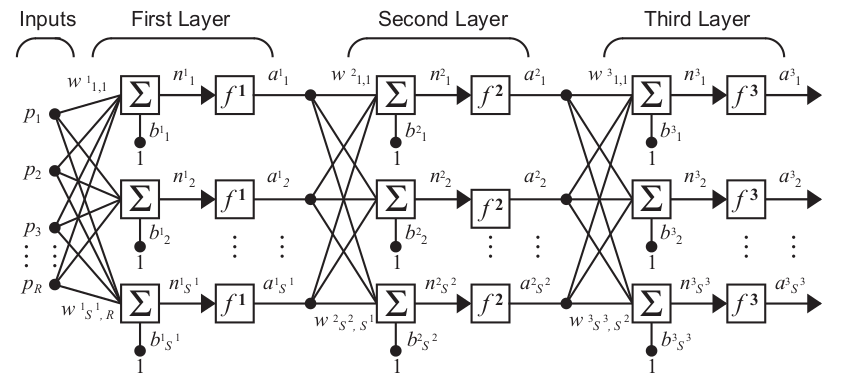
\includegraphics[width=\textwidth]{images/neuralnetworkmodel.png}
\caption{Model of three-layer Artificial Neural Network}
\label{fig:neuralnetworkmodel}
\end{figure}

Denoting $\mathbf{p}$ as the $R\times 1$-dimensional input vector of
the whole network, $\mathbf{b}^1$ the $S\times 1$-dimensional bias
vector of the first layer and $\mathbf{W}^1$ as the $S\times
R$-dimensional matrix of weights of the same layer, the $S\times
1$-dimensional net input vector of that particular layer
$\mathbf{n}^1$ can be expressed as:
\begin{equation} 
\mathbf{n}^1=\mathbf{W}^1\mathbf{p}+\mathbf{b}^1
\label{eq:netinputvector}
\end{equation}

This way, \figref{neuralnetworkmodel} can we redrawn
as \figref{neuralnetworkmodelVectorial} and,
combining \esref{expandedgeneralneuroneq}{netinputvector}, the
$S\times 1$-dimensional output vector of the whole network
$\mathbf{a}^3$ can be written as:

\begin{equation}
\mathbf{a}^3=\mathbf{f}^3(\mathbf{W}^3\mathbf{f}^2(\mathbf{W}^2\mathbf{f}^1(\mathbf{W}^1\mathbf{p}+\mathbf{b}^1)+\mathbf{b}^2)+\mathbf{b}^3)
\label{eq:ouputnetworkvector}
\end{equation}

\begin{figure}[!ht]
\centering
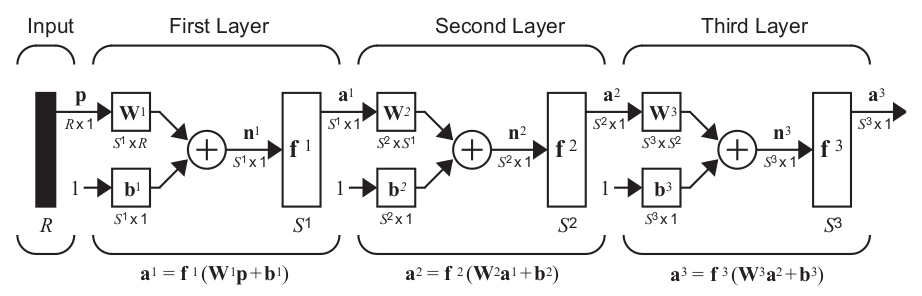
\includegraphics[width=\textwidth]{images/neuralnetworkmodelVectorial.png}
\caption{Model of three-layer Artificial Neural Network with matrix notation}
\label{fig:neuralnetworkmodelVectorial}
\end{figure}

It is important to highlight that, when implementing ANNs, the first
layer is called \emph{input layer}, the last one \emph{output layer}
and all the intermediate ones are known as \emph{hidden layers}.
%When there is no hidden layers, it is said that the net is a one-layer network. This way, two-layers networks will denote a net with a unique hidden layer. The reason of this is that the weigths of the input layer are usually fixed to $w=1$.

Now, if one looks at \figref{neuralnetworkmodel}, it is noticed that
the network drawn has no feedback elements and contains no delays in
any layer. This kind of networks are known as \emph{static
feedforward} nets, in which the output is calculated directly from the
input through feedforward connections.  In the others, classified
as \emph{dynamic} nets, the output depends not only on the current
input to the network, but also on the previous inputs
(\emph{feedforward-dynamic}) and outputs
(\emph{recurrent-dynamic}) \cite{dimith3neural}.  Because dynamic
networks have memory, they can be trained to learn sequential or
time-varying patterns, which is exactly what our project needs to
predict a migraine.


\subsection{Learning rules}
\label{subsec:learningrules}

As we indicated in \subsecref{neuronmodel}, the weights and the biases
parameters of each neuron can be adjusted so that the network
input/output relationship meets some specific goal.The procedure for
modifying these terms is known as \emph{learning} or \emph{training
algorithm}.

In general, training rules can be divided into two broad
categories \cite{demuth2008neural}:
\begin{itemize}
\item \emph{Supervised} or \emph{Associative learning}
, in which the network is trained by providing it with input and
target output patterns known as ``the training set''. Thus, a training
set of $Q$ patterns can be expressed as
\begin{equation}
\{\mathbf{p}_1,\mathbf{t}_1\},\{\mathbf{p}_2,\mathbf{t}_2\}, ... , \{\mathbf{p}_Q,\mathbf{t}_Q\}
\end{equation}
where $\mathbf{p}_q$ is an input vector of the network and
$\mathbf{t}_q$ is the corresponding target output vector.  The
learning rule is then used to adjust the weights and biases of the
network by comparing the network outputs and the targets when the
corresponding set of inputs are applied to the network.
\item \emph{Unsupervised} learning or \emph{Self-organisation}, in which there are no target outputs available, so the weights and biases are modified in response to network inputs only. 
Unlike the supervised learning, there is no a priori set of patterns
to be learn; rather the system must develop its own representation of
the input stimuli.
\end{itemize}

It is important to emphasize that, whichever is the learning rule
chosen for a particular ANN, the training begins by assigning some
initial values for the network parameters. Then, the corresponding
algorithm will be in charge of adjusting them to perform the desired
task.

Since our experimental scenario considers a target output (the pain
curve described in \secref{paincurve}), we have focused in the subset
of supervised training algorithms.  Among the available learning rules
of this type, the \emph{backpropagation} algorithm has been the centre
of our attention. It is a gradient-based learning rule that both
static an dynamic networks can use with minor changes. A complete
explanation of the backpropagation algorithm can be read
in \secref{generalbackprop}.


\subsection{Advantages and disadvantages}

% \textsc{COPY-PASTE!!!!!!!!!!!!!!!!!!!!!!!!!!!! - ESCRIBIR}\\
% Due to the admissible predictive performance of NN, it is presently the
% most popular data modeling method used in the medical domain [37]. The ability of the NN is to model
% highly nonlinear systems such as physiological records where the correlation of the input parameters is
% not easily detectable [71].

% In sum, since the progress of learning in NN would be complex, the method is commonly used for
% decision making in clinical conditions with large and complicated data sets. But same as SVM it could
% not handle domain knowledge to enrich the results. Additionally, as the modeling process in NN is a
% black box progress, NN method needs to justify for each input data. So, NN is not counted as a portable
% technique to easily apply for diverse data sets.

% Artificial neural networks were up until recently the
% most popular artificial intelligence-based data modeling
% algorithm used in clinical medicine. This is probably due to
% their good predictive performance, albeit they may have a
% number of deficiencies [18] that include high sensitivity to the
% parameters of the method—including those that determine
% the architecture of the network, high computational cost in
% training, and induction of the model that may – at best – be
% hard to interpret by domain experts. Neural networks may be
% able to model complex non-linear relationships, comprising
% an advantage over simpler modeling methods like the na ̈ve
% ı
% Bayesian classifier or logistic regression.

